\section{Experiments}
\label{sec:exp}

This section presents experimental results using our approach to debug
the circuits and perform a single-fix rectification. 
We compare results of our implementation against the incremental SAT-based approach presented in~\cite{fujita:2015} wherever it's relevant.
The approach presented in~\cite{fujita:2015} is implemented using PICOSAT~\cite{picosat}. The experiments were performed on a 3.5GHz 
Intel(R) $\text{Core}^{\text{TM}}$ i7-4770K Quad-Core CPU with 32 GB of RAM.

\begin{table*}[hbt]
\centering
\caption{{\footnotesize Single fix rectification debug in Mastrovito circuit against word level specification. Time is in seconds; $k$ = Datapath Size, \#Gates = No. of gates, K = $10^3$, \textit{a}=verification time, \textit{b}=time for rectification check, \textit{c}=time for component correction computation, \textit{d}=total time}}
\label{masvsspec}
\begin{tabular}{| c | c | c | c | c | c | c | c | c | c | c | c | c | c |} \hline
\multirow{3}{*}{\textbf{k}}& \multirow{3}{*}{\#Gates} & \multicolumn{12}{ c |}{Our implementation}\\ \cline{3-14}
&&\multicolumn{4}{ c |}{\it NI}&\multicolumn{4}{ c |}{\it NM}&\multicolumn{4}{ c |}{\it NO}\\ \hline
&&{\it a}&{\it b}&{\it c} &{\it d}&{\it a}&{\it b}&{\it c} &{\it d}&{\it a}&{\it b}&{\it c} &{\it d}\\ \hline
9 & 0.23K & 0.0 & 0.0 & 0.0 & 0.0 & 0.0 & 0.0 & 0.0 & 0.0 & 0.0 & 0.0 & 0.0  & 0.0\\ \hline
10& 0.29K & 0.0 & 0.0 & 0.0 & 0.0 & 0.0 & 0.0 & 0.0 & 0.0 & 0.0 & 0.0 & 0.0  & 0.0\\ \hline
11& 0.35K & 0.0 & 0.0 & 0.1 & 0.1 & 0.0 & 0.0 & 0.1 & 0.1 & 0.0 & 0.0 & 0.1  & 0.1\\ \hline
12& 0.97K & 0.1 & 0.5 & 0.4 & 0.9 & 0.2 & 0.5 & 0.4 & 1.1 & 0.5 & 0.8 & 0.4  & 1.7\\ \hline
13& 0.82K & 0.1 & 0.3 & 0.2 & 0.6 & 0.2 & 0.6 & 0.2 & 1.0 & 0.7 & 0.8 & 0.2  & 1.7\\ \hline
16& 1.8K  & 0.9 & 2.6 & 1.0 & 4.5 & 1.1 & 3.5 & 1.0 & 5.6 & 2.8 & 5.3 & 1.0  & 9.1\\ \hline
32& 5.4K  & 36  & 110 & 42  & 188 & 40  & 160 & 47  & 247 & 38  & 240 & 150  & 428\\ \hline
64& 21.8K & 2210& 7100 & 2432 & 9532 & 2200 & 8000 & 2575 & 12775 & 2150& 7840 & 10020 & 20010 \\ \hline
\end{tabular}
\end{table*}
% The data-path sizes {$k$} are selected according to cryptography standards recommended by U.S. National Institute of Standards and Technology (NIST). 
% In our experiments, the labels $NO$, $NM$, and $NI$ denote 
% % the location of unknown component within the circuit topology. Here $NI$, $NM$, and $NO$ 
% that the unknown component is near the input, middle, and near the output, respectively.
We have performed experiments for the cases when the bugs  are present near 
the input, middle, or near the output of the circuit, represented
using labels $NI$, $NM$, and $NO$ respectively in the tables. All the algorithms
were implemented in SINGULAR~\cite{DGPS}. 

%\subsection{Word level specification v/s Gate level implementation}

\subsubsection{Verification between a word level specification v/s Mastrovito implementation}
~\autoref{masvsspec} presents the results of our approach when the bugs are placed
in a Mastrovito multiplier implementation compared against a specification, which is given in terms of a word level polynomial $f$. 
A Mastrovito multiplier has word level specification $Z = A\times B \pmod{ P(x)}$, 
where $P(x)$ is a given primitive polynomial for the datapath size $k$. 
% The product $A \times B$ is computed using an array multiplier architecture, and then the result is reduced modulo $P(x)$. 
Bugs in the circuit are introduced, and the presence of the bugs is
detetced. Then we apply our approach to check for single-fix
rectification interatively on the nets selected in $\mathcal{N}$. If
rectification is feasible at $x_i$, the unknown component problem is
solved to identify a rectification function. 

%% The circuit implementation is modeled as a set of polynomials $F=\{f_1,\dots f_i,\dots,f_s\}$. The 
%% approach then follows the partial reduction of specification polynomial $f$ until leading term of $f_i$ while
%% recording the intermediate quotients and remainders. We then represent the partial remainder as a linear combination
%% using the remaining gate polynomials and the quotient to obtain the solution $P$.
We are able to verify and debug the circuits for upto 64-bits within our
stipulated Time Out ($TO$)  period.

% \begin{table}[H]
% \centering
% \caption{{Single fix rectification debug in Mastrovito circuit against word level specification}. Time is in seconds; $k$ = Datapath Size, \#Gates = No. of gates, K = $10^3$}
% \label{masvsspec}
% \begin{tabular}{| c | c | c | c | c | c | c | c | c | c | c | c | c | c | c | c | c |} \hline
% \multirow{3}{*}{\textbf{k}}& \#Gates & \multicolumn{15}{ c |}{Our implementation}\\ \cline{3-17}
% &&\multicolumn{5}{ c |}{\it NI}&\multicolumn{5}{ c |}{\it NM}&\multicolumn{5}{ c |}{\it NO}\\ \hline
% &&{\it a}&{\it b}&{\it c} &{\it d}&{\it e}&{\it a}&{\it b}&{\it c} &{\it d}&{\it e}&{\it a}&{\it b}&{\it c} &{\it d}&{\it e}\\ \hline
% 9& 0.23K & 0.0 & 0.1 & 0.0 & 0.2 & 0.0 & 0.1 & 0.0 & 0.2 & 0.0 & 0.2 & 0.0 & 0.3\\ \hline
% 10& 0.29K & 0.0 & 0.3 & 0.0 & 0.3 & 0.0 & 0.3 & 0.0 & 0.3 & 0.0 & 0.4 & 0.0 & 1.4\\ \hline
% 11& 0.35K & 0.0 & 0.2 & 0.0 & 0.3 & 0.0 & 0.3 & 0.0 & 0.4 & 0.0 & 0.6 & 0.0 & 0.7\\ \hline
% 12& 0.97K & 0.1 & 7.5 & 0.5 & 8.0 & 0.2 & 10.1 & 0.5 & 10.5 & 0.5 & 121.2 & 0.8 & 121.3\\ \hline
% 13& 0.82K & 0.1 & 4.3 & 0.3 & 4.5 & 0.2 & 11.3 & 0.6 & 11.2 & 0.7 & 156.3 & 0.8 & 158.1\\ \hline
% 16& 1.8K & 0.9 & 14.1 & 2.6 & 30.2 & 1.1 & 33.1 & 3.5 & 34.9 & 2.8 & 501.2 & 5.3 & 503.0\\ \hline
% 32& 5.4K & 36.8 & 378.6 & 110.5 & 544.7 & 40.0 & 567.1 & 160.3 & 767.2 & 38.1 & 1286.1 & 240.3 & 1342.7\\ \hline
% %64& 21.8K & 36.8 & 378.6 & 110.5 & 544.7 & 40.0 & 567.1 & 160.3 & 767.2 & 38.1 & 1286.1 & 240.3 & 1342.7\\ \hline
% \end{tabular}
% \end{table}

\subsubsection{Word level specification v/s Point addition implementation}
Point addition is an operation required for the task of encryption, decryption 
and authentication in Elliptic Curve Cryptography (ECC). 
Modern approaches represent the points in projective
coordinate systems, {\it e.g.}, the L$\acute{o}$pez-Dahab (LD) projective coordinate, due to which the point addition 
operation can be implemented as polynomials in the field.

\begin{Example}
  %Consider point addition in L$\acute{o}$pez-Dahab (LD) projective
  %coordinate.
  Given an elliptic curve: $Y^2 + XYZ = X^3Z + aX^2Z^2 +
  bZ^4$ over $\mathbb{F}_{2^k}$, where $X,Y,Z \in \mathbb{F}_{2^k}$ and similarly, $a, b$ are
  constants from the field. Point addition over the
  elliptic curve is ($X_3$, $Y_3$, $Z_3$) = ($X_1$, $Y_1$, $Z_1$) +
  ($X_2$, $Y_2$, $1$).  Then $X_3$, $Y_3$, $Z_3$ can be computed as
  follows:
% {
% \vspace{-0.40in}
\begin{align*}
&A = Y_2 \cdot Z_1^2 + Y_1  &&B = X_2 \cdot Z_1 + X_1 \\
&C = Z_1 \cdot B  &&D = B^2 \cdot(C + a Z_1^2) \\
&Z_3 = C^2 && E = A \cdot C  \\
&X_3 = A^2 + D + E &&F = X_3 + X_2 \cdot Z_3 \\
&G = X_3 + Y_2\cdot Z_3 && Y_3 = E\cdot F + Z_3 \cdot G
\end{align*}
% }
\end{Example}
% \vspace{-0.1in}
Each of the polynomials in the above design are implemented as a
(gate-level) logic block and are interconnected to obtain final
outputs $X_3,Y_3$ and $Z_3$. ~\autoref{pdvsspec} shows
the comparison of the time required for debugging and rectification
for the implementation of the block $D= B^2\cdot(C + aZ_1^2)$. 
\\
\begin{table}[H]
\centering
\caption{{\footnotesize Single fix rectification debug in Point Addition circuits against word level specification. Time is in seconds; $k$ = Datapath Size, \#Gates = No. of gates, K = $10^3$, \textit{a}=verification time, \textit{b}=time for rectification check, \textit{c}=time for component correction computation, \textit{d}=total time}}
\label{pdvsspec}
\begin{tabular}{| c | c | c | c | c | c | c | c | c | c | c | c | c | c |} \hline
\multirow{3}{*}{\textbf{k}}& \multirow{3}{*}{\#Gates} & \multicolumn{12}{ c |}{Our implementation}\\ \cline{3-14}
&&\multicolumn{4}{ c |}{\it NI}&\multicolumn{4}{ c |}{\it NM}&\multicolumn{4}{ c |}{\it NO}\\ \hline
&&{\it a}&{\it b}&{\it c} &{\it d}&{\it a}&{\it b}&{\it c} &{\it d}&{\it a}&{\it b}&{\it c} &{\it d}\\ \hline
8 & 244  & 0.0 & 0.0 & 0.0 & 0.0 & 0.0 & 0.0 & 0.0 & 0.0 & 0.0 & 0.0 & 0.0 & 0.0\\ \hline
16& 1.2K & 1.3 & 3.9 & 1.5 & 6.7 & 1.2 & 3.7 & 2   & 6.9 & 1.2 & 3.7 & 1.8 & 6.7\\ \hline
32& 3.9K & 37  & 112 & 77  & 226 & 38  & 110 & 22  & 170 & 37  & 108 & 35  & 180\\ \hline
%64& 15K  & 40  & 2283&  &  &  &  &  &  &  &  &   & \\ \hline
\end{tabular}
\end{table}

\subsubsection{Word level specification v/s Barrett reduction implementation}
Barrett reduction
%~\cite{barrett}
is the other widely used multiplier design
method adopted in cryptography system designs. 
Based on Barrett reduction, a multiplier can be designed in two steps:
multiplication $R = A \times B$ and a subsequent Barrett reduction G =
R (mod P). ~\autoref{bartvsspec} shows results for debugging and rectification of
Barrett multipliers against a polynomial specification. 
\\
\begin{table}[H]
\centering
\caption{{\footnotesize Single fix rectification debug in Barrett reduction circuits against word level specification. Time is in seconds; $k$ = Datapath Size, \#Gates = No. of gates, K = $10^3$, \textit{a}=verification time, \textit{b}=time for rectification check, \textit{c}=time for component correction computation, \textit{d}=total time}}
\label{bartvsspec}
\begin{tabular}{| c | c | c | c | c | c | c | c | c | c | c | c | c | c |} \hline
\multirow{3}{*}{\textbf{k}}& \multirow{3}{*}{\#Gates} & \multicolumn{12}{ c |}{Our implementation}\\ \cline{3-14}
&&\multicolumn{4}{ c |}{\it NI}&\multicolumn{4}{ c |}{\it NM}&\multicolumn{4}{ c |}{\it NO}\\ \hline
&&{\it a}&{\it b}&{\it c} &{\it d}&{\it a}&{\it b}&{\it c} &{\it d}&{\it a}&{\it b}&{\it c} &{\it d}\\ \hline
8 & 134 & 0.0 & 0.0 & 0.0 & 0.0 & 0.0 & 0.0 & 0.0 & 0.0 & 0.0 & 0.0 & 0.0 & 0.0\\ \hline
16& 427 & 0.1 & 0.0 & 0.0 & 0.1 & 0.0 & 0.2 & 0.1 & 0.3 & 0.0 & 0.1 & 0.3 & 0.4\\ \hline
32& 1.4K & 0.4 & 1.4 & 0.1 & 1.9 & 0.5 & 1.5 & 0.1 & 2.1 & 1.2 & 2.2 & 1.1 & 4.5\\ \hline
64& 4.9K & 19  & 58  & 5.4 & 82  & 21  & 60  & 1.7 & 83  & 63  & 104 & 141 & 308\\ \hline
\end{tabular}
\end{table}

Since the SAT-based approach cannot be applied against a word level specification polynomial, 
we perform experiments while using another multiplier implementation as the specification.

\subsubsection{Verification between a specification and implementation
  given as gate level circuits: Mastrovito v/s Montgomery multipliers}
\begin{table*}[hbt]
\centering
\caption{{\footnotesize Rectification for Mastrovito circuit with Montgomery circuit as specification. Time is in seconds; $k$ = Datapath Size, \#Gates = No. of gates, (TO): Time-Out = 3 hrs, K = $10^3$, \textit{a}=verification time, \textit{b}=time for rectification check, \textit{c}=time for component correction computation, \textit{d}=total time}}
\label{masusmontspec}
\begin{tabular}{| c | c |  c | c | c | c | c | c | c | c | c | c | c | c | c | c | c |} \hline
\multirow{4}{*}{\textbf{k}}& \multirow{4}{*}{\#Gates} & \multicolumn{3}{ c |}{Incremental SAT\textbf{~\cite{fujita:2015}}}& \multicolumn{12}{ c |}{Our Approach}\\ \cline{3-17}
&&\multirow{2}{*}{\it NI}&\multirow{2}{*}{\it NM}&\multirow{2}{*}{\it NO}&\multicolumn{4}{ c |}{\it NI}&\multicolumn{4}{ c |}{\it NM}&\multicolumn{4}{ c |}{\it NO} \\ \cline{6-17}
&&&&&{\it a}&{\it b}&{\it c} &{\it d}&{\it a}&{\it b}&{\it c} &{\it d}&{\it a}&{\it b}&{\it c} &{\it d}\\ \hline
9 & 0.6K & 35   & 37   & 33    & 0.1 & 0.5 & 0.2 & 0.8 & 0.2 & 0.2 & 0.1 & 0.5 & 1.8 & 2.2 & 0.6 & 4.6 \\ \hline
10& 0.7K & 231  & 215  & 214   & 0.3 & 1   & 0.5 & 1.8 & 0.3 & 1   & 0.8 & 2.1 & 4.7 & 5.4 & 0.2 & 10 \\ \hline
11& 0.9K & 2090 & 1927 & 2000  & 0.6 & 2   & 1   & 3.6 & 0.8 & 2   & 32  & 35  & 9 & 10 & 0.4 & 19 \\ \hline
12& 1.6K & 8676 & 23400& 24085 & 3.2 & 9.6 & 3.5 & 16  & 3.2 & 9.3 & 12  & 24  & 155 & 160 & 1.6 & 316 \\ \hline
13& 1.7K & TO   & TO   & TO    & 3.3 & 10  & 4.5 & 18  & 3.5 & 10 & 22 & 35 & 170 & 177 & 1.6 & 349 \\ \hline
16& 3K   & TO   & TO   & TO    & 27  & 81  & 35  & 143 & 28 & 83 & 48 & 159 & 210 & 176 & 2.5 & 389\\ \hline
32& 9.8K & TO   & TO   & TO    &  2060   & 6595    & 1870&  10525   & 2100 & 7320 & 1289 & 10709 & 2215 & 7870 & 1204 & 11289 \\ \hline
\end{tabular}
\end{table*} 
%% \begin{table*}[ht]
%% \centering
%% \caption{{Resolving Unknown Component in Mastrovito circuit with Montgomery circuit as specification}. Time is in seconds; $k$ = Datapath Size, \#Gates = No. of gates, (TO): Time-Out = 3 hrs, K = $10^3$,\textit{a}=verification time, \textit{b}=time for rectification check,\textit{c}=time for component correction computation,\textit{d}=total time}
%% \label{masusmontspec}
%% \begin{tabular}{| c | c |  c | c | c | c | c | c | c | c | c | c | c | c | c | c | c |} \hline
%% \multirow{4}{*}{\textbf{k}}& \multirow{4}{*}{\#Gates} & \multicolumn{3}{ c |}{Incremental SAT\textbf{~\cite{fujita:2015}}}& \multicolumn{12}{ c |}{Our Approach}\\ \cline{3-17}
%% &&\multirow{2}{*}{\it NI}&\multirow{2}{*}{\it NM}&\multirow{2}{*}{\it NO}&\multicolumn{4}{ c |}{\it NI}&\multicolumn{4}{ c |}{\it NM}&\multicolumn{4}{ c |}{\it NO} \\ \cline{6-17}
%% &&&&&{\it a}&{\it b}&{\it c} &{\it d}&{\it a}&{\it b}&{\it c} &{\it d}&{\it a}&{\it b}&{\it c} &{\it d}\\ \hline
%% 9 & 0.6K & 35   & 37   & 33    & 0.1 & 0.5 & 0.2 & 0.8 & 0.2 & 0.2 & 0.1 & 0.5 & 1.8 & 2.2 & 0.6 & 4.6 \\ \hline
%% 10& 0.7K & 231  & 215  & 214   & 0.3 & 1   & 0.5 & 1.8 & 0.3 & 1   & 0.8 & 2.1 & 4.7 & 5.4 & 0.2 & 10 \\ \hline
%% 11& 0.9K & 2090 & 1927 & 2000  & 0.6 & 2   & 1   & 3.6 & 0.8 & 2   & 32  & 35  & 9 & 10 & 0.4 & 19 \\ \hline
%% 12& 1.6K & 8676 & 23400& 24085 & 3.2 & 9.6 & 3.5 & 16  & 3.2 & 9.3 & 12  & 24  & 155 & 160 & 1.6 & 316 \\ \hline
%% 13& 1.7K & TO   & TO   & TO    & 3.3 & 10  & 4.5 & 18  & 3.5 & 10 & 22 & 35 & 170 & 177 & 1.6 & 349 \\ \hline
%% 16& 3K   & TO   & TO   & TO    & 27  & 81  & 35  & 143 & 28 & 83 & 48 & 159 & 210 & 176 & 2.5 & 389\\ \hline
%% 32& 9.8K & TO   & TO   & TO    &     &     & 1870&     &  &  & 1289 &  &  &  & 1204 &  \\ \hline
%% \end{tabular}
%% \end{table*}

%\subsubsection{Mastrovito v/s Montgomery}
%% \begin{figure}[H]
%%   \centering
%%   %\def\svgwidth{340pt}
%%   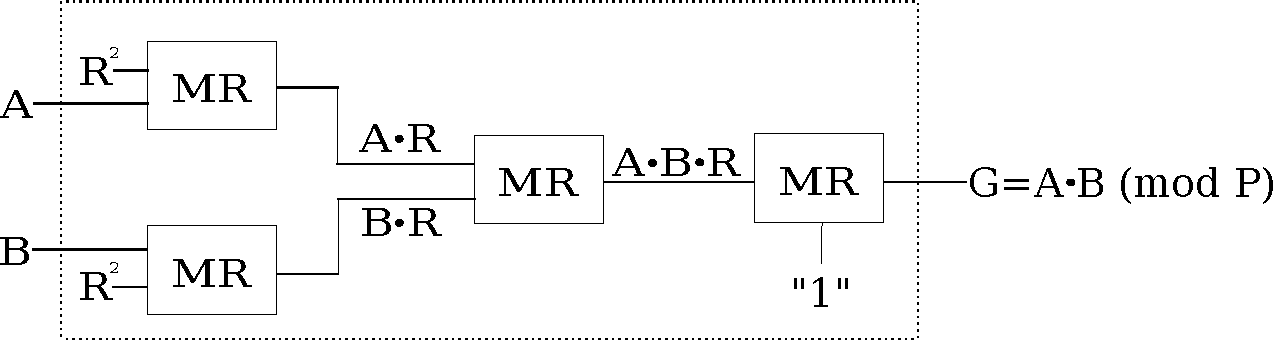
\includegraphics[scale=0.34]{new_mmcircuit-eps-converted-to}
%%   \caption{Montgomery multiplication.}
%%   \label{montfig}
%%   \end{figure}

Montgomery architectures~\cite{acar:1998}
% ,~\cite{wu:2002},
% \cite{Barrett:1987} 
% ~\cite{knezevic:2008} 
are considered more efficient than Mastrovito multipliers for exponentiation, 
as they do not require explicit reduction modulo $P(x)$ after each step.
%% ~\autoref{montfig} shows the structure of a Montgomery
%% multiplier. Each MR block computes $A\cdot B\cdot R^{-1}$, where $R$
%% is selected as a power of a base ($\alpha^{k}$) and $R^{-1}$ is the multiplicative 
%% inverse of $R$ in $\mathbb{F}_{2^k}$. As this operation cannot compute $A\cdot B$
%% directly, we need to pre-compute $A\cdot R$ and $B\cdot R$ as shown in the~\autoref{montfig}. 
%% We denote the leftmost
%% two blocks as Block A (upper) and B (lower), the middle block as Block
%% C and the output block as Block D.
% We have presented results for GBR
%on both \textit{flattened} and \textit{hierarchical} netlists of these
% multipliers.

~\autoref{masusmontspec} presents the results of our approach to debug
and rectification with the bugs placed in the Montgomery multiplier
with a Mastrovito multiplier circuit used as the specification. While
the approach~\cite{fujita:2015} finds a satisfying transformation
assignment which can be mapped to a library gate, our approach debugs
the circuit and finds a single fix rectification function. As shown in
the table, our approach shows improvement by several orders of
magnitude over \cite{fujita:2015}. 

%The comparison of bug placement reflects the complexity involved in
%debugging circuits where the bug lies in the deeper part ($NO$) of the
%topology.
It takes considerable amount of time for verification and
rectification check when the bug is close to the output. We are
working on further improving the experiments by employing better data
structures like  
ZBDDs~(\cite{minato:zbdd}), and devising better heuristics to perform
rectification check.
%We are also looking into efficient
%implementations for representing the partial remainder as a linear
%combination of an ideal during correction computation.
Due to several limitations w.r.t the number of ring variables that can be
declared in SINGULAR, we have had to restrict our experiments within
64-bit data-path size.   

\section{Conclusions}

This paper has presented a fully automated debug approach for single fix 
rectification of finite field arithmetic circuits. 
% The gates of the circuit C are modeled as a set of polynomials where the variables 
% are the nets of the circuit. An order on the variables is derived from 
% the topology of the circuit, and a lex term order (RTTO $>$) is imposed on the polynomials. 
Given a specification and its circuit implementation, we verify the circuit. 
If verification detects a bug, we identify all potential single-fix rectification target nets, 
and perform rectification check at each of these nets. If a net admits single-fix rectification, 
we compute a corresponding rectification function. 
The underlying theory and algorithms are based on \Grobner basis reductions, Nullstellensatz, and ideal membership test.  
The experimental results demonstrate the efficacy of our approach for finite field 
arithmetic circuits where we achieve several orders of magnitude
improvement as compared to recent SAT-based approach. 
As part of our future work, we are working on improving the efficiency of our 
implementation to target higher bit-widths. We are also investigating how the 
current procedure can be extended to cover integer arithmetic circuits.
Further research also includes exploring the current approach for
the case of multi-fix rectification.  
